\documentclass[12pt, varwidth, border=5mm]{standalone}
\usepackage{tikz}
\usepackage{amsmath}
% Underlining package
\usepackage{ulem}
\usetikzlibrary{calc}
\usetikzlibrary{angles,quotes}
% \usepackage[a4paper, portrait, margin=1cm]{geometry}

\begin{document}
\section*{ }
    \begin{minipage}{0.55\textwidth}
  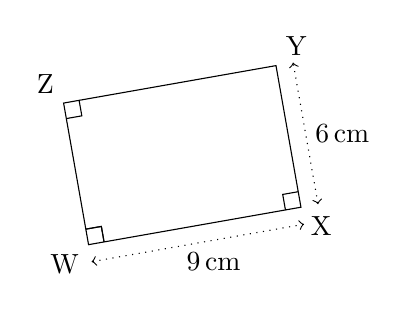
\begin{tikzpicture}[scale=1.1, baseline=(current bounding box.north)]
    \begin{scope}[rotate=10]
        % Draw square
        \draw (0,0) coordinate (W) --
              ++(2.49,0) coordinate (X) --
              ++(0,1.66) coordinate (Y) --
              ++(-2.49,0) coordinate (Z) -- cycle;

        % Right angle markers
        \foreach \p/\q/\r in {Z/W/X,W/X/Y,Y/Z/W,Z/W/X} {
            \pic [draw, -, angle radius=0.2cm] {right angle=\p--\q--\r};
        }

        % Vertex LABELS
        \foreach \p/\l in {W/below left,X/below right,Y/above right,Z/above left} {
            \node[\l] at (\p) {\p};
        }

        % Dotted arrows shifted away from edges
        % Horizontal side (A-B), shifted down
        \draw[<->, dotted]
            ($(W) + (0,-0.2cm)$) -- ($(X) + (0,-0.2cm)$)
            node[midway,below, xshift=2mm] {9\,cm};

        % Vertical side (B-C), shifted right
        \draw[<->, dotted]
            ($(X) + (0.2cm,0)$) -- ($(Y) + (0.2cm,0)$)
            node[midway,right] {6\,cm};
    \end{scope}
\end{tikzpicture}
\end{minipage}%
\hfill
\begin{minipage}{.4\textwidth}
  \begin{align*}
  \text{Area} &= lw \\
  \text{Area} &= 9 \,\text{cm} \times 6 \,\text{cm} \\
  \text{Area} &= 54 \,\text{cm}^2
  \end{align*}
\end{minipage}

\end{document}
